%\documentclass[handout]{beamer}
\documentclass[]{beamer}
\usetheme[]{Boadilla}
%\usepackage{pgfpages}
%\pgfpagesuselayout{2 on 1}[a4paper,border shrink=5mm]

\usepackage{float}
\usepackage{graphicx}
\usepackage{subfig}

\title{Logical Neural Networks}
\subtitle{Opening The Black Box\\
\vspace{0.5cm}
\small COMP 489 Project
}
\author{Daniel Braithwaite}
\date{Supervisor: Marcus Frean}

\begin{document}

\begin{frame}
\titlepage
\end{frame}

\begin{frame}
\frametitle{Introduction + Motivation}

\begin{figure}
\centering
	\begin{minipage}[b]{0.8\textwidth}
		
\includegraphics[width=\textwidth]{Images/BlackBox.png}
	\end{minipage}
	\hfill
\end{figure}

 Difficult to interpret Artificial Neural Networks using standard activations, e.g., Sigmoid, TanH.

\begin{block}{Why Interpretable Systems?}
\begin{itemize}
\item Safety Critical Systems
\item Ensuring systems make Ethical decisions
\item European Union General Data Protection Regulation
\end{itemize}
\end{block}
\end{frame}

\begin{frame}
\frametitle{Problem Statement}

\begin{itemize}
\item Want Artificial Neural Networks which can achieve a high accuracy.
\item Want Artificial Neural Networks which have an interpretable learned model so their predictions can be defended
\end{itemize}

\end{frame}

\begin{frame}
\frametitle{Idea}

\begin{itemize}
\item Some problems appear to have a logical decomposition 
\item Logical functions are a natural thing for humans to interpret
\item \textbf{Goal:} Learn these logical decompositions using Backpropagation
\item \textbf{Problem:} Standard Boolean Logic Gates are not continuous.
\end{itemize}

\begin{figure}
\centering
	\begin{minipage}[b]{0.2\textwidth}
		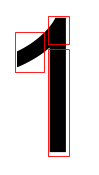
\includegraphics[width=\textwidth]{Images/DigitDecomp.png}
	\end{minipage}
	\hfill
\end{figure}


\end{frame}

\begin{frame}
\frametitle{Noisy-OR Relation}

\begin{figure}
\centering
	\begin{minipage}[b]{0.4\textwidth}
		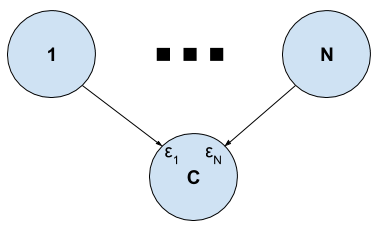
\includegraphics[width=\textwidth]{Images/NoisyOR.png}
	\end{minipage}
	\hfill
\end{figure}

\begin{itemize}
\item Every parent is on, but there exsists uncertanty as to node $i$ influences the child.
\item $\epsilon_i \in [0,1]$ is the probability that input $i$ is irrelevant to C. 
\item $C = OR(x_1, ..., x_n)$, so $P(C = 0 | x_i = 1 \forall i) = 0$ 
\item What if there is uncertainty that input $i$ influences C. Then $P(C = 0 | x_i = 1 \forall i) = \prod P(C = 0 | x_i = 1)$
\item Therefore $P(C = 1 | x_i = 1 \forall i) = 1 - \prod \epsilon_i$
\end{itemize}

\end{frame}

\begin{frame}
\frametitle{Noisy Neurons}

\begin{figure}
\centering
	\begin{minipage}[b]{0.4\textwidth}
		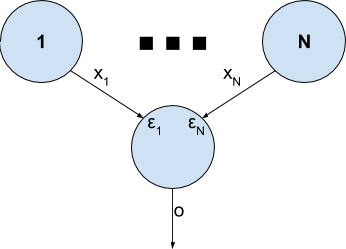
\includegraphics[width=\textwidth]{Images/NoisyNeuronEG.png}
	\end{minipage}
	\hfill
\end{figure}

\begin{itemize}
\item Noisy-OR relation almost gives the OR activation we are looking for.
\item Insted each input node will be on with probability $x_i$.
\item The total irrelevence of the node $i$ is then defined as $\epsilon_i^{x_i}$
\item The Noisy-OR activation is therefore $1 - \prod_{\forall i} \epsilon_i^{x_i}$
\item In a similar fassion the Noisy-AND activation is given as $\prod_{\forall i} \epsilon_i^{1 - x_i}$
\item Both activations reduce to descrete gates when inputs are binary and $\epsilon_i = 0$.
\end{itemize}


\end{frame}

\begin{frame}
\frametitle{Approach: Logical Neural Networks}
Logical Neural Networks have layers consisting of Noisy Neurons. Can be trained with Backpropagation.

\begin{block}{Problem: Weight Initialization}
\begin{itemize}
\item Even small networks would not train.
\item Derived a distribution from which to sample weights.
\item Now large networks can be trained, including deep Logical Networks. Up to 10 layers deep were tested!
\end{itemize}
\end{block}

\end{frame}

\begin{frame}
\frametitle{Experimental Approach}

\begin{itemize}
\item Want to evaluate accuracy and interpretability of Logical Neural Networks
\item Implement in Tensorflow.
\item Logical Neural Networks are compared against Multi Layer Perceptron Networks (of equivelent size) using the MNIST problem.
\item \textbf{Accuracy:} Networks trained from 30 different initial conditions, accuracy compared using confidence intervals obtained from evaluation of the network on a testing set.
\item \textbf{Interpretability:} Results are obtained by visually comparing interpretations of the weights from different networks.
\item It will be diffcult to give conclusive evidence given the experements are limited.
\end{itemize}
\end{frame}

\begin{frame}
\frametitle{Experimental Results: Accuracy}

\begin{itemize}
\item Logical Neural Networks have statistically equivalent accuracy to Multi-Layer Perceptron Networks.
\end{itemize}
\end{frame}

\begin{frame}
\frametitle{Experimental Results: Interpretability}
\begin{itemize}
\item Logical Neural Networks are potentially more interpretable that Multi-Layer Perceptron Networks.
\item Interpretability of Logical Neural Networks depends on activations used.
\end{itemize}
\end{frame}

\begin{frame}
\frametitle{Experimental Results: Interpretability - No Hidden}
Pictures represent the weights in learned the models, specifically the output neuron representing a 0. Dark regions are most important, and white is irrelevant.
%\begin{example}{Single Layer Networks}

%\begin{itemize}
%\item Perceptron Network
\begin{minipage}[t]{0.4\textwidth}
\begin{figure}[H]
	\centering
	\begin{minipage}[b]{0.7\textwidth}
		\captionsetup{labelformat=empty}
		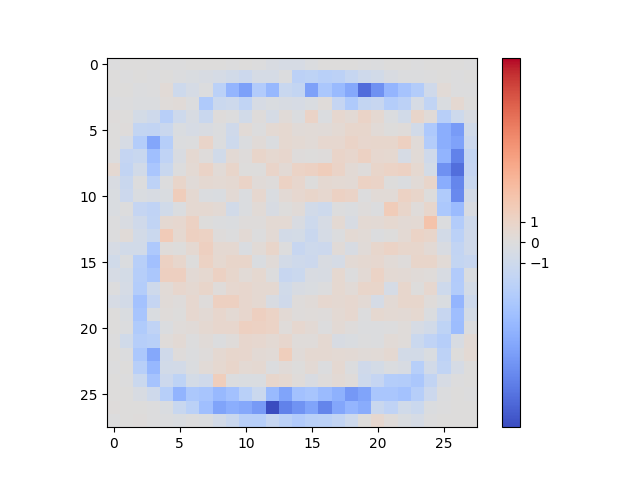
\includegraphics[width=\textwidth]{Images/Sigmoid(NO-Hidden)/Layer0-Neuron-0.png}
		%\caption{Digit 0}
	\end{minipage}
	\caption{Features for a perceptron network}
	\hfill
\end{figure}
\end{minipage}
\hspace{0.1\textwidth}
\begin{minipage}[t]{0.4\textwidth}
\begin{figure}[H]
	%\captionsetup{labelformat=empty}
	\centering
	\begin{minipage}[b]{0.7\textwidth}
		\captionsetup{labelformat=empty}
		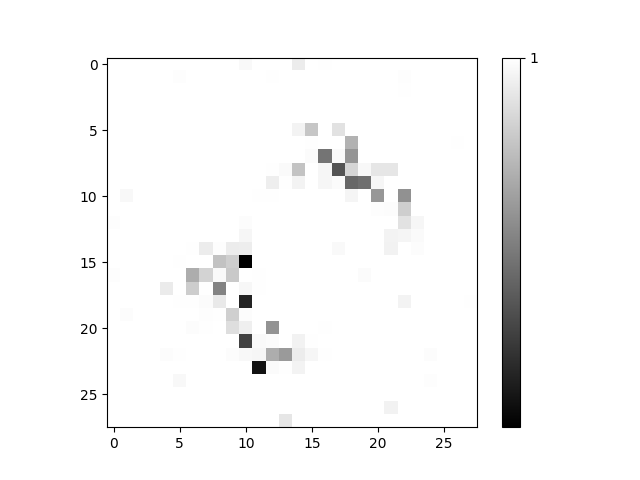
\includegraphics[width=\textwidth]{Images/AND(LSM)/Positive/Layer0-Neuron-0.png}
		%\caption{Digit 0}
	\end{minipage}
	
	\medskip

	\begin{minipage}[b]{0.7\textwidth}
		\captionsetup{labelformat=empty}
		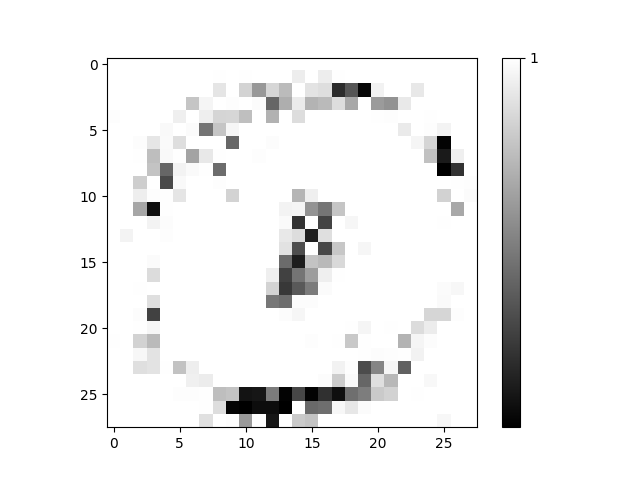
\includegraphics[width=\textwidth]{Images/AND(LSM)/Negative/Layer0-Neuron-0.png}
		%\caption{Not Digit 0}
	\end{minipage}
	\caption{Logical Neural Network using an AND activation}
	\hfill
\end{figure}
\end{minipage}
%\end{itemize}

%\end{example}
\end{frame}

\begin{frame}
\frametitle{Experimental Results: Interpretability - Hidden Layer}
In this case, pictures represent an important feature for classifying an instance as a 1.

\noindent
\begin{minipage}[t]{0.4\textwidth}
	\begin{figure}[H]
		\centering
		\begin{minipage}[b]{0.7\textwidth}
			\captionsetup{labelformat=empty}
			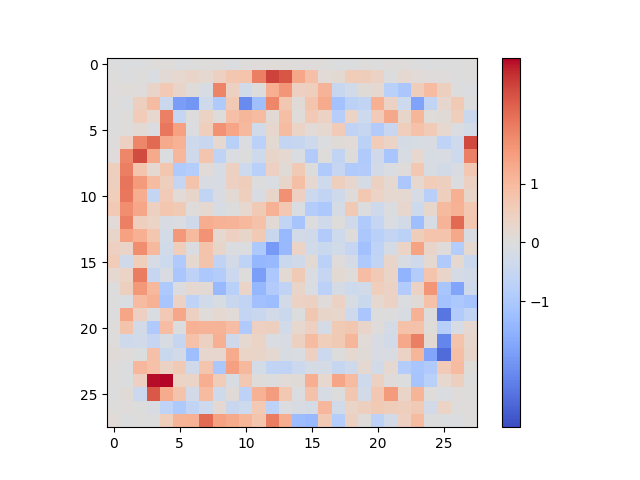
\includegraphics[width=\textwidth]{Images/Sigmoid(Hidden-Layer)/Like/Layer0-Neuron-11.png}
			%\caption{Digit 0}
			\label{}
		\end{minipage}
		\caption{Features that positively contribute to the classification as a 1.}
		\hfill
	\end{figure}
\end{minipage}
\hspace{0.1\textwidth}
\begin{minipage}[t]{0.4\textwidth}
\begin{figure}[H]
		\centering
		\begin{minipage}[b]{0.7\textwidth}
			\captionsetup{labelformat=empty}
			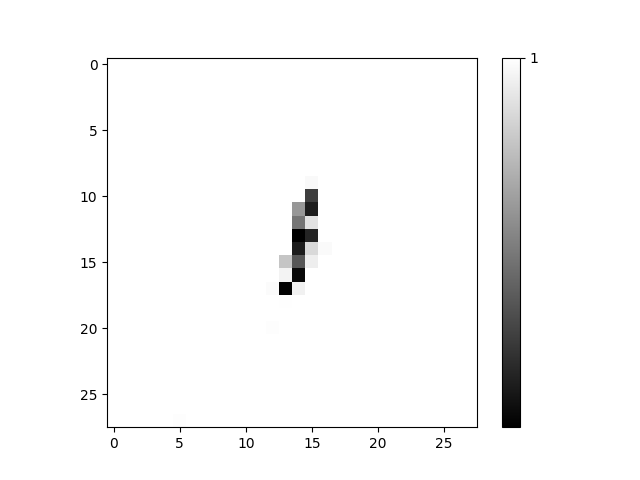
\includegraphics[width=\textwidth]{Images/AND-OR(W-LSM)(1)/Like/True/Layer0-Neuron-9.png}
			%\caption{Digit 0}
			\label{}
		\end{minipage}
		
		\medskip
		
		\begin{minipage}[b]{0.7\textwidth}
			\captionsetup{labelformat=empty}
			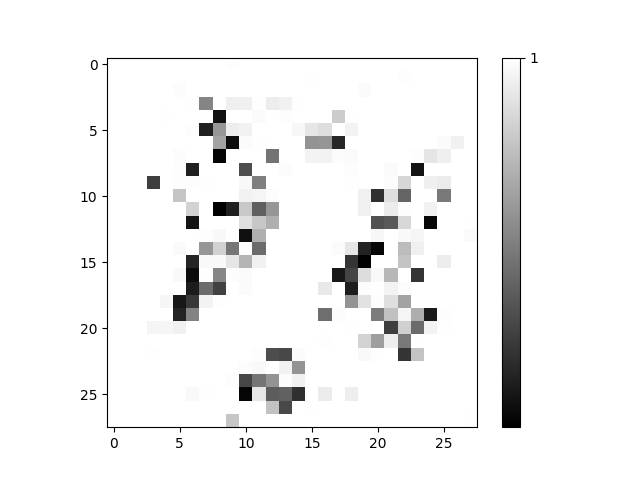
\includegraphics[width=\textwidth]{Images/AND-OR(W-LSM)(1)/Like/False/Layer0-Neuron-9.png}
			%\caption{Digit 0}
			\label{}
		\end{minipage}
		\caption{Features contributing to classification of a 1 in an  AND $\rightarrow$ OR Model}
		\hfill
	\end{figure}

\end{minipage}
\end{frame}

\begin{frame}
\frametitle{Conclusion}

\begin{block}{Did we succeed in solving the problem? Well... Yes and No}
\begin{itemize}
\item Logical Neural Networks are a promising alternative to Multi-Layer Perceptron Networks.
\item Interpretability on MNIST was "better". However, this is difficult to establish.
\item Can train shallow and deep networks with good accuracy.
\end{itemize}
\end{block}
\end{frame}

\begin{frame}
\begin{center}
\huge Questions
\end{center}
\end{frame}

\end{document}